We present a method that allows compressing any sized CM ($d,w$) to any new size possible ($d,w'$) for $w' \in [1,w]$. 
Let $h_1, \dots ,h_d$ be \inblue{pair-wise independent} hash functions used in original CM, such that every function holds $h_i : \{f_1,f_2, \dots\} \mapsto \{1,2, \dots, w\}$, \inblue{where $f_j$ is flow $j$}. Let $g_1,...,g_d$ be \inblue{pair-wise independent} hash functions such that $g_i : \{1,2, \dots, w\} \mapsto \{1,2, \dots, w'\}$ for every $i$. 

The CM-SKTC compression method works as follows. For each array $\textsl{S}^c[j]$ in the sketch, the value of the $l$'s cell $\textsl{S}^c[j][l]$ is the maximum value over all cells in the corresponding array of the original sketch $\textsl{S}[j]$ that by the hash function $g_j$ are hashed to the $l$'th cell (i.e. $\textsl{S}^c[j][l] \gets \max\limits_{i: g_j(i) = l} \{ \textsl{S}[j][i]\}$). Algorithm~\ref{sktc-alg:w-compression} presents the CM-SKTC compression method pseudo code.

An example of the compression process of CM-SKTC is illustrated in Figure \ref{sktc-fig:cm-sktc-example} where a CM-SKTC of size  $d=2, w'=4$ is computed for a CM of size $d=2, w=6$. Notice that the method reduces the number of columns (rather than that of the rows) since typically the number of rows is low beforehand, as there is a need for a distinct hash function per row.

The query method (Algorithm \ref{sktc-alg:w-compression-query}) from CM-SKTC is similar to the original CM query. When flow $f$ estimation value is required, for each array $\textsl{S}^c[j]$ (where $j \in [1,d]$) find the appropriate cell  $\textsl{S}^c[j][g_j\left(h_j(f)\right)]$ (one in each array) and return their respective minimal value. 

%One can see that as Zip sketch cannot create an under-estimated result,  
Similar to the original CM and the \textbf{MM}~\cite{yang2018elastic},  the CM-SKTC method also generates only overestimation values. 

\begin{algorithm}[h]
    \small
    \begin{algorithmic}[1]
    \Statex vars:
    \Statex $h_1,\dots h_d$ - hash functions from flows to $[1,w]$
    \Statex $g_1, \dots g_d$ - hash functions from $[1,w]$ to $[1,w']$
        \Procedure{compress}{$S$}
        \State $S^c \gets $ array of $0$'s of size $d \times w'$
        \For{$j \in [1 \dots d]$}
        \For{$i \in [1 \dots w]$}
        \State $l \gets g_j(i)$
        \State  $S^c[j][l] = \max(S^c[j][l], S[j][i])$
      \EndFor
      \EndFor
      \State \Return $S^c$
        \EndProcedure

    \end{algorithmic}
    \caption{CM-SKTC compression algorithm}
    \label{sktc-alg:w-compression}
\end{algorithm}

% Change the algorithm to be O(wd) instead of O(w'dw)
% \setlength{\textfloatsep}{2pt}
% \begin{algorithm}[t!]
% \begin{algorithmic}[1]
% 		\REQUIRE{A CM \textsl{S}  (size $d \times w$), new width $w'$}
% 		\ENSURE{Compressed CM-SKTC \textsl{S}$^c$ with size $d \times w'$}
		
% 		\STATE $\textsl{S}^c \gets $ array of $0$'s of size $d \times w'$
% 		\FOR{$j=1; \ j\leq d;\ j++$}
%             \FOR{$i=1; \ i\leq w;\ i++$}
%                 \STATE $l=g_j(i)$
%                 \STATE  $S^c[j][l] = \max(S^c[j][l], S[j][i])$ 
%   %             \IF{$S[j][i] > S^c[j][l]$}
% %                    \STATE $S^c[j][l] = S[j][i]$
% %                \ENDIF
%             \ENDFOR
%         \ENDFOR
% 		\RETURN $\textsl{S}^c$
% 	\end{algorithmic}
% 	\caption{CM-SKTC compression algorithm}
% 	\label{sktc-alg:w-compression}
% \end{algorithm}

\begin{figure}[t!]
    \centering
    

\tikzset{every picture/.style={line width=0.75pt}} %set default line width to 0.75pt        

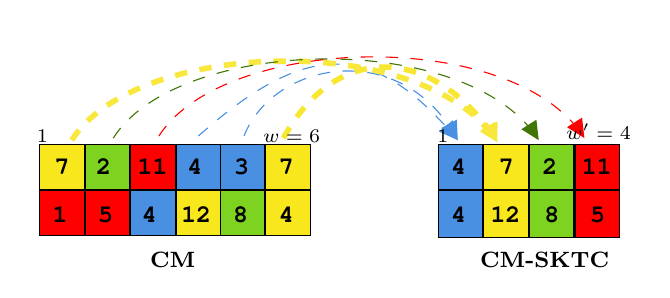
\begin{tikzpicture}[x=0.75pt,y=0.75pt,yscale=-1,xscale=1]
%uncomment if require: \path (0,300); %set diagram left start at 0, and has height of 300

%Shape: Rectangle [id:dp9120519996767289] 
\draw  [fill={rgb, 255:red, 248; green, 231; blue, 28 }  ,fill opacity=1 ] (39,134) -- (60.5,134) -- (60.5,156) -- (39,156) -- cycle ;
%Shape: Rectangle [id:dp5578762422129069] 
\draw  [fill={rgb, 255:red, 126; green, 211; blue, 33 }  ,fill opacity=1 ] (61,134) -- (82.5,134) -- (82.5,156) -- (61,156) -- cycle ;
%Shape: Rectangle [id:dp5149322189764962] 
\draw  [fill={rgb, 255:red, 255; green, 0; blue, 0 }  ,fill opacity=1 ] (83,134) -- (104.5,134) -- (104.5,156) -- (83,156) -- cycle ;
%Shape: Rectangle [id:dp8371364169912505] 
\draw  [fill={rgb, 255:red, 74; green, 144; blue, 226 }  ,fill opacity=1 ] (105,134) -- (126.5,134) -- (126.5,156) -- (105,156) -- cycle ;
%Shape: Rectangle [id:dp8774137890100953] 
\draw  [fill={rgb, 255:red, 74; green, 144; blue, 226 }  ,fill opacity=1 ] (126,134) -- (147.5,134) -- (147.5,156) -- (126,156) -- cycle ;
%Shape: Rectangle [id:dp8260064759507215] 
\draw  [fill={rgb, 255:red, 248; green, 231; blue, 28 }  ,fill opacity=1 ] (148,134) -- (169.5,134) -- (169.5,156) -- (148,156) -- cycle ;
%Shape: Rectangle [id:dp13750697143490287] 
\draw  [fill={rgb, 255:red, 255; green, 0; blue, 0 }  ,fill opacity=1 ] (39,156) -- (60.5,156) -- (60.5,178) -- (39,178) -- cycle ;
%Shape: Rectangle [id:dp12750267479029076] 
\draw  [fill={rgb, 255:red, 255; green, 0; blue, 0 }  ,fill opacity=1 ] (61,156) -- (82.5,156) -- (82.5,178) -- (61,178) -- cycle ;
%Shape: Rectangle [id:dp9453531436538745] 
\draw  [fill={rgb, 255:red, 74; green, 144; blue, 226 }  ,fill opacity=1 ] (83,156) -- (104.5,156) -- (104.5,178) -- (83,178) -- cycle ;
%Shape: Rectangle [id:dp019183616299335293] 
\draw  [fill={rgb, 255:red, 248; green, 231; blue, 28 }  ,fill opacity=1 ] (105,156) -- (126.5,156) -- (126.5,178) -- (105,178) -- cycle ;
%Shape: Rectangle [id:dp9174572360745898] 
\draw  [fill={rgb, 255:red, 126; green, 211; blue, 33 }  ,fill opacity=1 ] (126,156) -- (147.5,156) -- (147.5,178) -- (126,178) -- cycle ;
%Shape: Rectangle [id:dp2814590512908379] 
\draw  [fill={rgb, 255:red, 248; green, 231; blue, 28 }  ,fill opacity=1 ] (148,156) -- (169.5,156) -- (169.5,178) -- (148,178) -- cycle ;
%Shape: Rectangle [id:dp3867673825425666] 
\draw  [fill={rgb, 255:red, 74; green, 144; blue, 226 }  ,fill opacity=1 ] (231,134) -- (252.5,134) -- (252.5,157) -- (231,157) -- cycle ;
%Shape: Rectangle [id:dp45900611803416114] 
\draw  [fill={rgb, 255:red, 248; green, 231; blue, 28 }  ,fill opacity=1 ] (253,134) -- (274.5,134) -- (274.5,157) -- (253,157) -- cycle ;
%Shape: Rectangle [id:dp14536752724329527] 
\draw  [fill={rgb, 255:red, 126; green, 211; blue, 33 }  ,fill opacity=1 ] (275,134) -- (296.5,134) -- (296.5,157) -- (275,157) -- cycle ;
%Shape: Rectangle [id:dp7559601744598143] 
\draw  [fill={rgb, 255:red, 255; green, 0; blue, 0 }  ,fill opacity=1 ] (297,134) -- (318.5,134) -- (318.5,157) -- (297,157) -- cycle ;
%Shape: Rectangle [id:dp5499444494363386] 
\draw  [fill={rgb, 255:red, 74; green, 144; blue, 226 }  ,fill opacity=1 ] (231,156) -- (252.5,156) -- (252.5,179) -- (231,179) -- cycle ;
%Shape: Rectangle [id:dp6548836133040838] 
\draw  [fill={rgb, 255:red, 248; green, 231; blue, 28 }  ,fill opacity=1 ] (253,156) -- (274.5,156) -- (274.5,179) -- (253,179) -- cycle ;
%Shape: Rectangle [id:dp5995721454141998] 
\draw  [fill={rgb, 255:red, 126; green, 211; blue, 33 }  ,fill opacity=1 ] (275,156) -- (296.5,156) -- (296.5,179) -- (275,179) -- cycle ;
%Shape: Rectangle [id:dp8157813465457489] 
\draw  [fill={rgb, 255:red, 255; green, 0; blue, 0 }  ,fill opacity=1 ] (297,156) -- (318.5,156) -- (318.5,179) -- (297,179) -- cycle ;
%Curve Lines [id:da7793812944008702] 
\draw [color={rgb, 255:red, 74; green, 144; blue, 226 }  ,draw opacity=1 ] [dash pattern={on 4.5pt off 4.5pt}]  (115.5,130) .. controls (166.72,84.69) and (198.54,83.04) .. (238.66,129.83) ;
\draw [shift={(240.5,132)}, rotate = 230.07999999999998] [fill={rgb, 255:red, 74; green, 144; blue, 226 }  ,fill opacity=1 ][line width=0.08]  [draw opacity=0] (8.93,-4.29) -- (0,0) -- (8.93,4.29) -- cycle    ;
%Curve Lines [id:da17576300112648635] 
\draw [color={rgb, 255:red, 74; green, 144; blue, 226 }  ,draw opacity=1 ] [dash pattern={on 4.5pt off 4.5pt}]  (137.5,130) .. controls (151.29,94.54) and (211.65,82.37) .. (239.26,129.79) ;
\draw [shift={(240.5,132)}, rotate = 241.63] [fill={rgb, 255:red, 74; green, 144; blue, 226 }  ,fill opacity=1 ][line width=0.08]  [draw opacity=0] (8.93,-4.29) -- (0,0) -- (8.93,4.29) -- cycle    ;
%Curve Lines [id:da12939079412155663] 
\draw [color={rgb, 255:red, 248; green, 231; blue, 50 }  ,draw opacity=2 ] [dash pattern={on 4.5pt off 4.5pt}][line width=2]  (156.5,131) .. controls (181.25,85.65) and (226.58,85.07) .. (258.54,130.92) ;
\draw [shift={(259.5,133)}, rotate = 245.43] [fill={rgb, 255:red, 248; green, 231; blue, 60 }  ,fill opacity=1 ][line width=0.5]  [draw opacity=0] (8.93,-4.29) -- (0,0) -- (8.93,4.29) -- cycle    ;
%Curve Lines [id:da23437502293589474] 
\draw [color={rgb, 255:red, 248; green, 231; blue, 60 }  ,draw opacity=1, line width=0.5 ] [dash pattern={on 4.5pt off 4.5pt}][line width=2]  (54.5,132) .. controls (85.04,83.73) and (221.32,79.13) .. (257.9,130.61) ;
\draw [shift={(259.5,133)}, rotate = 237.8] [fill={rgb, 255:red, 248; green, 231; blue, 60 }  ,fill opacity=1 ][line width=0.5]  [draw opacity=0] (8.93,-4.29) -- (0,0) -- (8.93,4.29) -- cycle    ;
%Curve Lines [id:da16470429934928688] 
\draw [color={rgb, 255:red, 65; green, 117; blue, 5 }  ,draw opacity=1 ] [dash pattern={on 4.5pt off 4.5pt}]  (74.5,131) .. controls (105.04,82.73) and (241.32,78.13) .. (277.9,129.61) ;
\draw [shift={(279.5,132)}, rotate = 237.8] [fill={rgb, 255:red, 65; green, 117; blue, 5 }  ,fill opacity=1 ][line width=0.08]  [draw opacity=0] (8.93,-4.29) -- (0,0) -- (8.93,4.29) -- cycle    ;
%Curve Lines [id:da3875594417212562] 
\draw [color={rgb, 255:red, 255; green, 0; blue, 0 }  ,draw opacity=1 ] [dash pattern={on 4.5pt off 4.5pt}]  (96.5,130) .. controls (124.04,86.47) and (237.6,78.45) .. (286.45,115.07) .. controls (291.73,119.02) and (296.25,123.5) .. (299.83,128.51) ;
\draw [shift={(301.5,131)}, rotate = 237.8] [fill={rgb, 255:red, 255; green, 0; blue, 0 }  ,fill opacity=1 ][line width=0.08]  [draw opacity=0] (8.93,-4.29) -- (0,0) -- (8.93,4.29) -- cycle    ;

% Text Node
\draw (44,163) node [anchor=north west][inner sep=0.75pt]  [font=\large,color={rgb, 255:red, 0; green, 0; blue, 0 }  ,opacity=1 ] [align=left] {{\fontfamily{pcr}\selectfont \textbf{{\small 1}}}};
% Text Node
\draw (66,163) node [anchor=north west][inner sep=0.75pt]  [font=\large,color={rgb, 255:red, 0; green, 0; blue, 0 }  ,opacity=1 ] [align=left] {{\fontfamily{pcr}\selectfont {\small \textbf{5}}}};
% Text Node
\draw (87,163) node [anchor=north west][inner sep=0.75pt]  [font=\large,color={rgb, 255:red, 0; green, 0; blue, 0 }  ,opacity=1 ] [align=left] {{\fontfamily{pcr}\selectfont {\small \textbf{4}}}};
% Text Node
\draw (106,163) node [anchor=north west][inner sep=0.75pt]  [font=\large,color={rgb, 255:red, 0; green, 0; blue, 0 }  ,opacity=1 ] [align=left] {{\fontfamily{pcr}\selectfont {\small \textbf{12}}}};
% Text Node
\draw (131,163) node [anchor=north west][inner sep=0.75pt]  [font=\large,color={rgb, 255:red, 0; green, 0; blue, 0 }  ,opacity=1 ] [align=left] {{\fontfamily{pcr}\selectfont {\small \textbf{8}}}};
% Text Node
\draw (153,163) node [anchor=north west][inner sep=0.75pt]  [font=\large,color={rgb, 255:red, 0; green, 0; blue, 0 }  ,opacity=1 ] [align=left] {{\fontfamily{pcr}\selectfont {\small \textbf{4}}}};
% Text Node
\draw (236,163) node [anchor=north west][inner sep=0.75pt]  [font=\large,color={rgb, 255:red, 0; green, 0; blue, 0 }  ,opacity=1 ] [align=left] {{\fontfamily{pcr}\selectfont {\small \textbf{4}}}};
% Text Node
\draw (255,163) node [anchor=north west][inner sep=0.75pt]  [font=\large,color={rgb, 255:red, 0; green, 0; blue, 0 }  ,opacity=1 ] [align=left] {{\fontfamily{pcr}\selectfont {\small \textbf{12}}}};
% Text Node
\draw (281,163) node [anchor=north west][inner sep=0.75pt]  [font=\large,color={rgb, 255:red, 0; green, 0; blue, 0 }  ,opacity=1 ] [align=left] {{\fontfamily{pcr}\selectfont {\small \textbf{8}}}};
% Text Node
\draw (303,163) node [anchor=north west][inner sep=0.75pt]  [font=\large,color={rgb, 255:red, 0; green, 0; blue, 0 }  ,opacity=1 ] [align=left] {{\fontfamily{pcr}\selectfont {\small \textbf{5}}}};
% Text Node
\draw (45,140) node [anchor=north west][inner sep=0.75pt]  [font=\large,color={rgb, 255:red, 0; green, 0; blue, 0 }  ,opacity=1 ] [align=left] {{\fontfamily{pcr}\selectfont \textbf{{\small 7}}}};
% Text Node
\draw (153,140) node [anchor=north west][inner sep=0.75pt]  [font=\large,color={rgb, 255:red, 0; green, 0; blue, 0 }  ,opacity=1 ] [align=left] {{\fontfamily{pcr}\selectfont \textbf{{\small 7}}}};
% Text Node
\draw (65,140) node [anchor=north west][inner sep=0.75pt]  [font=\large,color={rgb, 255:red, 0; green, 0; blue, 0 }  ,opacity=1 ] [align=left] {{\fontfamily{pcr}\selectfont \textbf{{\small 2}}}};
% Text Node
\draw (85,140) node [anchor=north west][inner sep=0.75pt]  [font=\large,color={rgb, 255:red, 0; green, 0; blue, 0 }  ,opacity=1 ] [align=left] {{\fontfamily{pcr}\selectfont \textbf{{\small 11}}}};
% Text Node
\draw (131.5,140) node [anchor=north west][inner sep=0.75pt]  [font=\large,color={rgb, 255:red, 0; green, 0; blue, 0 }  ,opacity=1 ] [align=left] {{\fontfamily{pcr}\selectfont \textbf{{\small 3}}}};
% Text Node
\draw (109,140) node [anchor=north west][inner sep=0.75pt]  [font=\large,color={rgb, 255:red, 0; green, 0; blue, 0 }  ,opacity=1 ] [align=left] {{\fontfamily{pcr}\selectfont \textbf{{\small 4}}}};
% Text Node
\draw (280,140) node [anchor=north west][inner sep=0.75pt]  [font=\large,color={rgb, 255:red, 0; green, 0; blue, 0 }  ,opacity=1 ] [align=left] {{\fontfamily{pcr}\selectfont \textbf{{\small 2}}}};
% Text Node
\draw (236,140) node [anchor=north west][inner sep=0.75pt]  [font=\large,color={rgb, 255:red, 0; green, 0; blue, 0 }  ,opacity=1 ] [align=left] {{\fontfamily{pcr}\selectfont \textbf{{\small 4}}}};
% Text Node
\draw (299,140) node [anchor=north west][inner sep=0.75pt]  [font=\large,color={rgb, 255:red, 0; green, 0; blue, 0 }  ,opacity=1 ] [align=left] {{\fontfamily{pcr}\selectfont \textbf{{\small 11}}}};
% Text Node
\draw (259,140) node [anchor=north west][inner sep=0.75pt]  [font=\large,color={rgb, 255:red, 0; green, 0; blue, 0 }  ,opacity=1 ] [align=left] {{\fontfamily{pcr}\selectfont \textbf{{\small 7}}}};

\draw (91,185) node [anchor=north west][inner sep=0.75pt]   [align=left] {\textbf{{\footnotesize CM}}};
\draw (250,185) node [anchor=north west][inner sep=0.75pt]   [align=left] {\textbf{{\footnotesize CM-SKTC}}};

\node[text width=0.5cm, anchor=west, right] at (33,130) {\scriptsize $1$};
\node[text width=0.85cm, anchor=west, right] at (142,130) {\scriptsize $w=6$};
\node[text width=0.5cm, anchor=west, right] at (226,130) {\scriptsize $1$};
\node[text width=0.85cm, anchor=west, right] at (288,128) {\scriptsize $w'=4$};

%\node[text width=0.5cm, anchor=west, right] at (1.31,1.90) {\scriptsize $1$};
%\node[text width=0.5cm, anchor=west, right] at (1.25,0.32) {\scriptsize $d$};
\end{tikzpicture}

    \caption{An example for Count-Min sketch (CM) (left side) compression with CM-SKTC (right side). In this example, a CM of size $d=2, w=6$ is compressed into a CM-SKTC of size  $d=2, w'=4$. Values of the hash functions $g_1, g_2$ are represented by various colors. In row $i$, multiple counters with the same hash value of $g_i$ are represented by their maximum.}
    \label{sktc-fig:cm-sktc-example}
\end{figure}

\begin{algorithm}[htb]
    \small
    \begin{algorithmic}[1]
    \Statex vars:
    \Statex $h_1,\dots h_d$ - hash functions from flows to $[1,w]$
    \Statex $g_1, \dots g_d$ - hash functions from $[1,w]$ to $[1,w']$
        \Procedure{query}{$S^c, f$}
            \State $est \gets 0$
            \For{$j \in [1 \dots d]$}
        \If{$est > S^c[j][g_j\left(h_j(f)\right)]$}
        \State $est \gets S^c[j][g_j\left(h_j(f)\right)]$
        \EndIf
      \EndFor
      \State \Return $est$
        \EndProcedure

    \end{algorithmic}
    \caption{CM-SKTC estimation query}
    \label{sktc-alg:w-compression-query}
\end{algorithm}

% \begin{algorithm}[t!]
% \begin{algorithmic}[1]
% 		\REQUIRE{A compressed CM-SKTC $\textsl{S}^c$ (size $d \times w'$), a flow $f$}
% 		\ENSURE{An estimation of $f$}
% 		\RETURN $\min\limits_{j \in [1\dots d]} \left\{\textsl{S}^c[j][g_j\left(h_j(f)\right)]\right\}$
% \end{algorithmic}
% \caption{CM-SKTC estimation query}\label{sktc-alg:w-compression-query}
% \end{algorithm}


Yang et al.~\cite{yang2018elastic} present error bounds for compressing the CM when reducing $w$ to some divider $w'$ (i.e., $w=z\cdot w'$ for an integer $z$). The number of counters compressed to the same counter is fixed as $w / w'$. Our CM-SKTC, however, maps a variable number of counters to each counter using hashing. This number can vary among the counters in an array or among the arrays, thereby adding a taste of randomness. \inblue{Recall that in the CM sketch $\delta$ (the error probability) is a function of the number of columns and $\epsilon$ (the error) is a function of the number of rows. Our compression scheme reduces the number of columns, therefore, intuitively, the probability of estimating the flow size with error at most $\epsilon$ is reduced by some factor. In practice, given a probability $\delta$, the CM-SKTC is initialized with enough columns so that after compression the probability of estimating the flow size with at most error $\epsilon$ is greater than $1-\delta$. } \inred{Given a CM sketch with $d$ rows, and $w$ columns, and a compression ratio $w'/w$, Lemma~\ref{sktc-lmma:single-array-compression} presents the guarantees of the compressed sketch.}

\begin{lemma}
Given a CM $\textsl{S}$ with $d$ rows and $w$ columns, for appropriate parameters $(\epsilon, \delta')$, and a CM-SKTC  compression ratio $\frac{w'}{w} < 1$.
Let $N$ be the size of the stream and denote by  $\hat{f_i}$ the estimation of flow with size $f_i$.  
Denote by $\beta$ the term $$ \left(1-\left(1-\frac{1}{\epsilon w}\right)\left(1-\frac{N}{w(f_i+\epsilon N)}\right)^{\frac{w}{w'}-1+\sqrt{-2\ln(1-\delta)\frac{w}{w'}}}\right)^d.$$
The estimation $\hat{f}$ of flow $f$ satisfies 
$\hat{f} \leq f + \epsilon N$ with probability $1 - \beta -\delta'(1-\beta)$.
\label{sktc-lmma:single-array-compression}
\end{lemma}


\begin{proof}[\textbf{Proof of Lemma \ref{sktc-lmma:single-array-compression}}]
Following the compression, each counter in array $j \in [1,d]$ of \textsl{S}$^c$ is the maximum of all values of counters from \textsl{S}  mapped to this counter by the corresponding function from $g_j$. Since the $d$ arrays in \textsl{S}$^c$ are independent, we begin by analyzing each array error contribution by itself.
For some array, let denote by $X_l$ the number of cells that mapped to cell $l \in [1,w']$ in \textsl{S}$^c$. \inblue{As the hash functions map the domain $\{1,2,\dots, w\}$ uniformly to the range $\{1,2,\dots, w'\}$, $X_l$ is \inred{a random variable drawn from} a binomial distribution with $p = 1/w'$ and $n=w$.}
As $X_l$ is binomial, $e \triangleq E(X_l) = \frac{w}{w'}$. \inblue{We now bound the number of rows in the original CM sketch that map to the rows in the compressed sketch using the Chernoff bound:} 
\begin{flalign*}
&\text{Pr}\left(X_l > e+\sqrt{-2\ln(\sqrt[d]{1-\delta})e}\right)\\
&= \text{Pr}\left(X_l > \left(1+\sqrt{
-2\ln(\sqrt[d]{1-\delta}) / e
}\right)e\right)  \\
\stackrel{\text{Chernoff bound}}{\leq} &e^{-
\frac{\left(
\sqrt{
-2\ln(\sqrt[d]{1-\delta}) / e
}\right)^2r}
{2}}= e^{-\frac{-2\ln(\sqrt[d]{1-\delta})e}{2e}} \\
&= e^{\ln(\sqrt[d]{1-\delta})} = \sqrt[d]{1-\delta}.
\end{flalign*}
Let  $C = \left\lceil e+\sqrt{-2\ln(1-\sqrt[d]{1-\delta})e} \right\rceil$. Following the compression, each counter in \textsl{S}$^c$ is the maximum value of at least $C$  counters from \textsl{S} \inblue{with probability at most $\sqrt[d]{1-\delta}$}. 

We bound the error for a flow $f_i$, which is mapped to one counter in \textsl{S} and compressed with at most $C-1$ other counters to a new counter \inblue{with probability at least $1-\sqrt[d]{1-\delta}$}. Denote by $n_1,...,n_C$ the number of packets which do not belong to flow $f_i$, but are mapped to the $C$ counters mapped to counter \textsl{S}. From the CM sketch, $\text{C}(n_i) \leq \frac{N}{w}$ for every $n_i$.
Without loss of generality assume that $f_i$ is mapped to $n_1$. Conclude that the estimation $\hat{f}_i$ is 
%\begin{flalign*}
$\hat{f}_i = \max(n_1+f_i,n_2,...,n_C)$ and accordingly
% \begin{flalign*}
% \text{Pr}(\hat{f}_i \geq f_i + \epsilon N)\\ 
% =\text{Pr}(\max(n_1+a_i,n_2,\dots,n_C) \geq f_i + \epsilon N)  \\ 
% \leq 1 - \text{Pr}(\max(n_1+a_i,n_2,\dots,n_C) < f_i + \epsilon N)  \\ 
% =1 - \text{Pr}(n_1+f_i < f_i + \epsilon N)\cdot \prod\limits_{j=2}^C \text{Pr}(n_j < f_i + \epsilon N)  \\
% %\end{align*}
% %\begin{align*}
% = 1 - \text{Pr}(n_1 < \epsilon N) \cdot \prod\limits_{j=2}^C \text{Pr}(n_j < f_i + \epsilon N) \\
%  \stackrel{\text{Markov inequality}}{\leq} 1 - \left(1-\frac{E(n_1)}{\epsilon N}\right) \cdot \prod\limits_{j=2}^C \left(1-\frac{E(n_j)}{f_i + \epsilon N}\right) \\
% \leq  1- \left(1-\frac{1}{w\epsilon}\right)\left(1-\frac{N}{w(f_i+\epsilon N)}\right)^{C-1}
% \end{flalign*}
\begin{gather*}
\text{Pr}(\hat{f}_i \geq f_i + \epsilon N)\\ 
=\text{Pr}(\max(n_1+a_i,n_2,\dots,n_C) \geq f_i + \epsilon N)  \\ 
\leq 1 - \text{Pr}(\max(n_1+a_i,n_2,\dots,n_C) < f_i + \epsilon N)  \\ 
=1 - \text{Pr}(n_1+f_i < f_i + \epsilon N)\cdot \prod\limits_{j=2}^C \text{Pr}(n_j < f_i + \epsilon N) \\
%\end{align*}
%\begin{align*}
= 1 - \text{Pr}(n_1 < \epsilon N) \cdot \prod\limits_{j=2}^C \text{Pr}(n_j < f_i + \epsilon N)
\end{gather*}
\begin{gather*}
 \stackrel{\text{Markov inequality}}{\leq} 1 - \left(1-\frac{E(n_1)}{\epsilon N}\right) \cdot \prod\limits_{j=2}^C \left(1-\frac{E(n_j)}{f_i + \epsilon N}\right) \\
\leq  1- \left(1-\frac{1}{w\epsilon}\right)\left(1-\frac{N}{w(f_i+\epsilon N)}\right)^{C-1}
\end{gather*}

\inblue{As the hash functions are pairwise independent, we can use this bound to bound the error of $\hat{f}_i$, the estimation of flow $f_i$. By definition $\hat{f}_i = \min(\hat{f}_i^1,\hat{f}_i^2,\dots,\hat{f}_i^d)$.}

\begin{flalign*}
&\text{Pr}(\hat{f}_i \geq f_i + \epsilon N) = \text{Pr}(\min(\hat{f}_i^1,\dots,\hat{f}_i^d) \geq f_i + \epsilon N) \\
&\leq \prod\limits_{j=1}^d \text{Pr}(\hat{f}_i^j \geq f_i + \epsilon N)
\end{flalign*}

We have shown that for any $j$: $\text{Pr}(\hat{f}_i^j \geq f_i + \epsilon N) \leq 1- \left(1-\frac{1}{w\epsilon}\right)\left(1-\frac{N}{w(f_i+\epsilon N)}\right)^{C-1}$, with probability $\delta' = \sqrt[d]{1-\delta}$. Therefore, \inblue{as the hash functions as pair-wise independent,} we can conclude that the following holds with probability of $\sqrt[d]{1-\delta}^d = 1-\delta$:
\begin{flalign*}
&\text{Pr}(\hat{f}_i \geq f_i + \epsilon N) \leq \prod\limits_{j=1}^d \text{Pr}(\hat{f}_i^j \geq f_i + \epsilon N)\\
&\leq \prod\limits_{j=1}^d 1- \left(1-\frac{1}{w\epsilon}\right)\left(1-\frac{N}{w(f_i+\epsilon N)}\right)^{C-1} \\
&= \left(1- \left(1-\frac{1}{w\epsilon}\right)\left(1-\frac{N}{w(f_i+\epsilon N)}\right)^{C-1}\right)^d = \beta. 
\end{flalign*}

With probability of $1-\delta$ the following holds: $\text{Pr}(\hat{f}_i \geq f_i + \epsilon N) \leq \beta$ , thus $\text{Pr}(\hat{f}_i \leq f_i + \epsilon N) \geq 1-\beta$ with probability \inblue{at least} $1-\delta$. Therefore the probability that $\hat{f}_i \leq f_i + \epsilon N$ is at least $(1-\delta)(1-\beta)=1-\beta-\delta(1-\beta)$.  
\end{proof}


\inblue{Lemma~\ref{sktc-lmma:single-array-compression} shows that \inred{compressing a sketch with parameter $\delta$ yields a sketch with parameter $\beta + \delta(1-\beta)$, where $\beta$ is as defined in the lemma. It follows that to achieve probability $\delta$ \textbf{after} compression, we must instantiate the uncompressed sketch with parameter $(\delta - \beta) / (1 - \beta)$.}
 Denote $\delta' = \beta + \delta(1-\beta)$. We empirically analyze how the compression affects the probability. Table~\ref{sktc-tbl:delta_tah} shows how $\delta'$ is affected by changes in $\delta$, $w' / w$, and $\epsilon$ respectively. $\delta'$ remains less than $3\delta$, therefore we initialize the CM sketch to have the number of columns for $3\delta$ as opposed to $\delta$. As the number of columns is $\lceil\ln 1/\delta \rceil$, generally, we need to add a single column in order for the error probability after compression to be less than $\delta$.}

\begin{table}[b]
\inblue{
\caption{\inred{Error probabilities after compression, for values of $\delta$, $\epsilon$  and the resize factor, as defined by Lemma~\ref{sktc-lmma:single-array-compression}.}}
    \label{sktc-tbl:delta_tah}
    \begin{tabular}{|c|c|c|c|c|}
        \cline{2-5} 
        \multicolumn{1}{c}{Resize Factor} & \multicolumn{2}{|c|}{ $0.6$} & \multicolumn{2}{c|}{ $0.9$}\tabularnewline
        \cline{2-5} 
        \multicolumn{1}{c}{$\delta \quad \backslash \quad \epsilon$} & \multicolumn{1}{|c|}{ $\quad\; 0.02 \quad\;$} & \multicolumn{1}{c|}{$\quad\; 0.06 \quad\;$} & \multicolumn{1}{c|}{$\quad\; 0.02  \quad\;$} & \multicolumn{1}{c|}{$\quad\; 0.06 \quad\;$}\tabularnewline
        \hline
        $0.04$ & $0.0936$  & $0.1177$  & $0.0841$  & $0.0925$\tabularnewline
        \hline 
        $0.08$ & $0.1791$  & $0.217$  & $0.1648$ & $0.1808$\tabularnewline
        \hline
    \end{tabular}
}
\end{table}


%\begin{figure}
%    \centering
%    \includegraphics[width=0.9\columnwidth]{figures/new_delta.png}
%    \caption{$\delta'$ as a function of $\delta$.}
%    \label{sktc-fig:new_delta}
%\end{figure}

%\begin{figure}
%    \centering
%    \includegraphics[width=0.9\columnwidth]{figures/new_resize_factor.png}
%    \caption{$\delta'$ as a function of the resize factor.}
%    \label{sktc-fig:new_resize_factor}
%\end{figure}

%\begin{figure}
%    \centering
%    \includegraphics[width=0.9\columnwidth]{figures/new_epsilon.png}
%    \caption{$\delta'$ as a function of $\epsilon$.}
%    \label{sktc-fig:new_epsilon}
%\end{figure}